%\documentclass[a4paper]{article}
%% Language and font encodings
\documentclass[twocolumn,aps,prl]{revtex4-1}
\usepackage[utf8]{inputenc}
\usepackage[spanish, es-tabla]{babel}
\usepackage[T1]{fontenc}
\usepackage{amsmath}
\usepackage{siunitx}
\usepackage{multirow}
\usepackage{float}
\usepackage{enumitem} % enumerar

\sisetup{math-micro=\text{µ},text-micro=µ}

\usepackage[toc,page]{appendix}

%% Sets page size and margins
\usepackage[a4paper,top=1.5cm,bottom=2cm,left=1.7cm,right=1.7cm,marginparwidth=1.75cm]{geometry}

%% Sets caption text size(its bigger than text)
\usepackage{caption}
\captionsetup[figure]{font=small}
\usepackage{subcaption}

%% Useful packages
\usepackage{svg}
\usepackage{epstopdf}
\usepackage{amsmath}
\usepackage{graphicx}
% \usepackage[showframe]{geometry}% http://ctan.org/pkg/geometry
%\usepackage[colorinlistoftodos]{todonotes}
\usepackage[colorlinks=true, allcolors=blue]{hyperref}

\newcommand{\nstar}{n^*} 
\newcommand{\Nstar}{N^*} 

%%%%%%%%%%%%%%%%%%%%%%%%%%%%%%%%%%%%%%%%%%%%%%%%%%%%%%
%%%%%%%%%%%%%%%%%%%%%%%%%%%%%%%%%%%%%%%%%%%%%%%%%%%%%%
%%%%%%%%%%%%%%%%%%%%%%%%%%%%%%%%%%%%%%%%%%%%%%%%%%%%%%
%%%%%%%%%%%%%%%%%%%%%%%%%%%%%%%%%%%%%%%%%%%%%%%%%%%%%%
%%%%%%%%%%%%%%%%%%%%%%%%%%%%%%%%%%%%%%%%%%%%%%%%%%%%%%

\begin{document}

% ██   ██ ███████  █████  ██████
% ██   ██ ██      ██   ██ ██   ██
% ███████ █████   ███████ ██   ██
% ██   ██ ██      ██   ██ ██   ██
% ██   ██ ███████ ██   ██ ██████

\title{Practico 1}
\author{M. G. Aramayo}
\affiliation{Matematica de sistemas biologicos, Instituto Balseiro}

% \begin{abstract}
% Mete acá las conclusiones.
% \end{abstract}

\maketitle


% ███████╗██╗  ██╗ ██╗
% ██╔════╝╚██╗██╔╝███║
% █████╗   ╚███╔╝ ╚██║
% ██╔══╝   ██╔██╗  ██║
% ███████╗██╔╝ ██╗ ██║
% ╚══════╝╚═╝  ╚═╝ ╚═╝

\section{Resolucion Ej 1:}

Para este sistema discreto: 
$$n_{t+1} = f(n_t, K, r)= \frac{r n_t}{1+\frac{r-1}{K} n_t}$$, 

los puntos fijos $n^*$ se obtienen resolviendo la ecuación:

$$
n^* = f(n^*, K, r)
$$

Reemplazando:

$$
\nstar = \frac{r \nstar}{1+\frac{r-1}{K} \nstar}
$$


Resolvemos esta ecuación para $r\neq 1$ (donde hay dinámica):

$$
\nstar (r-1) (\nstar-K) = 0 \Rightarrow \left\lbrace ^{\nstar = K} _{\nstar = 0}  \right .
$$

Usando el siguiente criterio de estabilidad, proveniente de un analisis de pequeñas perturbaciones (Valido bajo las mismas hipotesis que permiten un desarrollo en series de Taylor), donde $n_{t+1} = f(n_t,r)$ representa el mapeo 1D y $\nstar$ el punto fijo a analizar:

$$
\begin{aligned}
|f_{n}\left(n^{*},r\right)| = |\lambda| &=\left\{\begin{array}{ll}
<1 & \text { Estable } \\
>1 & \text { Inestable } \\
=1 & \text { Marginalmente estable } \\
=0 & \text { Superestable }
\end{array}\right.
\end{aligned}
$$

Se obtiene que:

$$
|f_{n}\left(n^{*},r\right)|=\frac{K^{2} r}{(K+\nstar(r-1))^{2}}
$$

De analizar este expresion y analizar r=0 aparte, se obtiene lo que puede verse en la Fig. \ref{fig:estabilidad}.

%**********
\begin{figure}[ht!]
    \centering
    \begin{subfigure}[b]{0.45\linewidth}
        \centering
        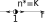
\includegraphics[width = 0.9\textwidth]{figuras/estabilidadK.pdf}
        \caption{}
        \label{fig:figuras/estabilidadK}
    \end{subfigure}\qquad
    \begin{subfigure}[b]{0.45\linewidth}
        \centering
        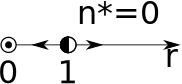
\includegraphics[width = 0.9\textwidth]{figuras/estable0.pdf}
        \caption{}
        \label{fig:figuras/estable0}
    \end{subfigure}\quad
    \caption{Estabilidad de los puntos fijos en segun el parametro $r$. El color negro indica el inicio de un intervalo de estabilidad y el blanco de un intervalo de inestabilidad. El circulo negro con marca blanca circular es un punto superestable.}
    \label{fig:estabilidad}
\end{figure}
%**********

En la Fig. \ref{fig:scripts/ex1} se tienen graficos de los mapeos. Se observa que dentro de un intervalo de estabilidad $r$ controla la velocidad de crecimiento de la poblacion. Hay dos casos particulares, si $r=1$ o $r=0$ no hay evolucion y $n=0$, $n=n_0$ son sus respectivos puntos superestables. 

% En la Fig. !!!! se tiene lo que ocurre para valores iniciales superiores a $K$, lo cual lleva a que el sistema se estabilice en $K$. 

\begin{figure*}[ht!]  
    \centering
    % \begin{subfigure}[b]{0.33\linewidth}
        \centering 
        \includegraphics[width = 0.99\textwidth]{scripts/ex1.pdf}
        \caption{Grafico del mapeo para distintos valores del parametro $r$, los puntos fijos se indican con linea punteada}
        \label{fig:scripts/ex1}
    % \end{subfigure}\quad
\end{figure*}

% \begin{equation}\label{eqn:etiqueta1}
%     \textit{Aca te metes alta ecuación bb}
% \end{equation}

% Acá te referencio la ecuación anterior, porque puedo, porque quiero y porque se me da la gana \ref{eqn:etiqueta1}.

% 
% ███████╗██╗  ██╗    ██████╗  
% ██╔════╝╚██╗██╔╝    ╚════██╗
% █████╗   ╚███╔╝      █████╔╝
% ██╔══╝   ██╔██╗     ██╔═══╝ 
% ███████╗██╔╝ ██╗    ███████╗
% ╚══════╝╚═╝  ╚═╝    ╚══════╝

\section{Resolucion Ej 2:}

\begin{figure}[ht!]
    \centering
    % \begin{subfigure}[b]{0.45\linewidth}
        \centering
        \includegraphics[width = 0.49\textwidth]{scripts/ex2-cosa.pdf}
        \caption{Soluciones de la ecuacion logistica con delay para tres valores del parametro $r$.}
        \label{fig:scripts/ex2-cosa}
    % \end{subfigure}\quad
\end{figure}

\begin{figure}[ht!]
    \centering
    % \begin{subfigure}[b]{0.33\linewidth}
        \centering
        \includegraphics[width = 0.49\textwidth]{scripts/ex2-aprox.pdf} 
        \caption{Grafico de soluciones ciclo limite para distintas condiciones inciales}
        \label{fig:scripts/ex2-aprox}
    % \end{subfigure}\quad
\end{figure}

\begin{figure}[ht!]
    \centering
    % \begin{subfigure}[b]{0.33\linewidth}
        \centering
        \includegraphics[width = 0.49\textwidth]{scripts/ex2-fourier-log.pdf}
        \caption{Transformada de Fourier del ciclo limite, para distintos valores de las condiciones iniciales.}
        \label{fig:scripts/ex2-fourier-log}
    % \end{subfigure}\quad
\end{figure}

\begin{figure}[ht!]
    \centering
    % \begin{subfigure}[b]{0.33\linewidth}
        \centering
        \includegraphics[width = 0.49\textwidth]{scripts/ex2-fourier-acotado.pdf}
        \caption{Transformada de Fourier del ciclo limite, puede verse que el periodo difiere de $4T$ en un 3\%.}
        \label{fig:scripts/ex2-fourier-acotado}
    % \end{subfigure}\quad
\end{figure}

En la Fig. \ref{fig:scripts/ex2-cosa} se tiene un gráfico de soluciones de la ecuacion logistica con delay. Estan presentes los 3 regímenes de la ecuación logística con Delay:

$$
\begin{array}{|l|l|}
\hline 0<r T <e^{-1} & \text { monótono } \\
e^{-1}<r T <\pi / 2 & \text { oscilatorio amortiguado } \\
\pi / 2<r T  & \text { ciclo límite } \\
\hline
\end{array}
$$





% 
% ███████╗██╗  ██╗    ██████╗     
% ██╔════╝╚██╗██╔╝    ╚════██╗    
% █████╗   ╚███╔╝      █████╔╝    
% ██╔══╝   ██╔██╗      ╚═══██╗    
% ███████╗██╔╝ ██╗    ██████╔╝    
% ╚══════╝╚═╝  ╚═╝    ╚═════╝     
%                                 
% 

\section{Resolucion Ej 3:}

Sea $R(r)$ la funcion polinomica:

\begin{equation}\label{eqn:etiqueta1}
    R(r) = r^{k+1} 
        - \left( 
            r^k f_0 
            - \sum_{l=1}^k 
            \left( 
            r^{k-l} f_l \prod_{j=0}^{l-1} s_j  
            \right) 
        \right)
\end{equation}

tal que $R(1)=R$. Puede verse que:

\begin{equation}\label{eqn:etiqueta2}
    R(0) = - f_k \cdot  s_{k-1} \cdot \ldots \cdot s_{0}
\end{equation}

Como es sabido, se cumple $f_j \geq 0, \forall \in \lbrace 0, \ldots, k \rbrace$, y sobre la supervivencia $  0 < s_j < 1, \forall \in \lbrace 0, \ldots, k - 1 \rbrace$.

Si se cumple que $f_k > 0$ se tiene que $R(0) < 0$. 

$R$ es un polinomio y por tanto una función continua. Por esto tiene tantos cambios de signo en su valor a lo largo de $r$ como raíces tenga $R$. 

El criterio de Descartes indica que esta raíz es positiva y hay solo una, sea $r_1$ esta raíz. Como hay una única raíz hay un único cambio de signo en $R$ respecto a $r$ en la recta real. 

Si se tiene que $R(0)$ y $R(1)$ son negativos y $r1>0$, se tiene que el cambio de signo ocurre después de estos valores. Es decir, la raíz no puede estar entre 0 y 1 porque eso implica que hay mas de un cambio de signo (uno para ir de $R(0)$ negativo a positivo y otro para volver al negativo en $R(1)$) como esto no es posible por el criterio de Descartes se tiene que $r1>1$.

% 
% ███████╗██╗  ██╗    ██╗  ██╗
% ██╔════╝╚██╗██╔╝    ██║  ██║
% █████╗   ╚███╔╝     ███████║
% ██╔══╝   ██╔██╗     ╚════██║
% ███████╗██╔╝ ██╗         ██║
% ╚══════╝╚═╝  ╚═╝         ╚═╝
%                             
% 

\section{Resolucion Ej 4:}

Se grafican en la Fig. \ref{fig:scripts/ex4} del mapeo con distintas semillas de números aleatorios. Las secuencias aleatorias de $r$ produce un rango amplio de máximos de población. Una secuencia de valores altos de r producen poblaciones enormes. Asimismo una racha de valores bajos resulta en la extinción de la población.

%**********
\begin{figure}[ht!]
    \centering
    % \begin{subfigure}[b]{0.33\linewidth}
        \centering
        \includegraphics[width = 0.45\textwidth]{scripts/ex4.pdf}
        \caption{Gráficos del mapeo con distintas semillas de números aleatorios. Una secuencia especifica de valores de $r$ produce un rango amplio de máximos de población.}
        \label{fig:scripts/ex4}
    % \end{subfigure}\quad
\end{figure}
%**********

% 
% ███████╗██╗  ██╗    ███████╗
% ██╔════╝╚██╗██╔╝    ██╔════╝
% █████╗   ╚███╔╝     ███████╗
% ██╔══╝   ██╔██╗     ╚════██║
% ███████╗██╔╝ ██╗    ███████║
% ╚══════╝╚═╝  ╚═╝    ╚══════╝
%                             
% 

\section{Resolucion Ej 5:}

%**********
\begin{figure*}[ht!]
    \centering
    \begin{subfigure}[b]{0.9\linewidth}
        \centering
        \includegraphics[width = 0.9\textwidth]{scripts/plots/ex5-02.pdf}
        \caption{}
        \label{fig:scripts/plots/ex5-02}
    \end{subfigure}\quad
% \end{figure*}
% \begin{figure*}[ht!]
%     \centering
    \begin{subfigure}[b]{0.9\linewidth}
        \centering
        \includegraphics[width = 0.9\textwidth]{scripts/plots/ex5-19.pdf}
        \caption{}
        \label{fig:scripts/plots/ex5-19}
    \end{subfigure}\quad
    \caption{Grafico del modelo !!! para distintos valores de $p$}
    \label{fig:scripts/plots/ex5}
\end{figure*}
%**********

Utilizando un modelo logístico interrumpido por "desastres" que perturban la solución con un parámetro $p$ tal que: $N(t^+)=pN(t)$. Con un tiempo medio entre desastres $1/\lambda$. Se resolvieron las ecuaciones para 20 valores distintos de p, en dos casos: $r = \text{1.01}, \lambda = \text{0.422}$ en Fig. \ref{fig:scripts/plots/ex5-02} (Caso a) y $r = \text{1.01}, \lambda = \text{0.422}$ \ref{fig:scripts/plots/ex5-19} (Caso b). Dentro de cada caso se utiliza la misma secuencia de eventos desastrosos para comparar el efecto del parametro $p$. En ambos casos se resolvio para 50 eventos desastrosos. 

Respecto a la dinamica se observo en el caso b que a medida que $p$ baja, la posibilidad de completar el crecimiento baja y la población empieza a crecer por debajo del punto fijo $K$. Se torna complicada la recuperación, para el caso a se observa que de las 20 curvas consideradas solo las 5 con el valor de $p$ mas alto sobreviven, en el resto de casos se llego a una extinción. 
En el caso b el tiempo medio de desastres $\lambda$ es mas corto que el tiempo de recuperación $1/r$, para este caso todos los valores de $p$ intentados se encuentran por debajo de $K$. Esto no ocurre en el caso a donde el tiempo medio de la ecuacion logistica es mas corto que el de la ocurrencia de desastres, por lo que la poblacion se recupera hasta el valor $K$ para 16 de los 20 valores de $p$ considerados. Con esto en cuenta, es posible que el sistema se recupere si $1/r > 1/\lambda$. Esto depende de $p$ porque aun para el caso a se observa una extincion en estas condiciones para $p =\text{0.05}$.

% 
% ███████╗██╗  ██╗     ██████╗ 
% ██╔════╝╚██╗██╔╝    ██╔════╝ 
% █████╗   ╚███╔╝     ███████╗ 
% ██╔══╝   ██╔██╗     ██╔═══██╗
% ███████╗██╔╝ ██╗    ╚██████╔╝
% ╚══════╝╚═╝  ╚═╝     ╚═════╝ 
%                              
% 

\section{Resolucion Ej 6:}

Para este sistema continuo:

$$
\frac{d N}{d t} =r N\left[1-\frac{N}{K}\right]\left[\frac{N}{A}-1\right] = f(N, K, r, A)
$$

$$
\frac{d N}{d t} = f(N, K, r, A) \qquad r>0, K>0 , A>0
$$

es conocido que los puntos fijos $N^*$ son las soluciones a la ecuación:

\begin{equation}\label{eqn:etiqueta3}
    0 = f(N^*, K, r, A), r>0, K>0, A >0
\end{equation}

Resolvemos esta ecuación para $r\neq 1$ (donde hay dinámica):

\begin{equation}\label{eqn:etiqueta3}
    - r \Nstar  (1 - \frac{\Nstar}{K}) (1 - \frac{\Nstar}{A}) = 0 \Rightarrow \left\lbrace ^{\Nstar = K, \Nstar = A} _{\Nstar = 0, }  \right .
\end{equation}

Usando el siguiente criterio de estabilidad, proveniente de un analisis de pequeñas perturbaciones (Valido bajo las mismas hipotesis que permiten un desarrollo en series de Taylor), donde $\frac{dN}{dt} = f(N, K, r, A)$ representa el sistema dinamico y $\Nstar$ el punto fijo a analizar:

$$
\begin{aligned}
    \frac{d f\left(x^{*}, r\right)}{d x} &=\left\{ 
        \begin{array}{ll}
            <0 & \text { Estable } \\
            >0 & \text { Inestable }
        \end{array}\right.
\end{aligned}
$$

Se tiene en este caso 3 puntos fijos pero hay 2 que estan "conectados", la forma del binomio es identica pero con distinto parametro, los puntos fijos son los ceros de la funcion.

Para $\frac{d f\left(x^{*}, r\right)}{d x} (0):$ 

$$\frac{d f\left(x^{*}, r\right)}{d x} (0) = -r \Rightarrow \text{Estable}$$ 

Para $\frac{d f\left(x^{*}, r\right)}{d x} (A):$ 

$$\frac{d f\left(x^{*}, r\right)}{d x} (A) = \frac{r}{K} (K-A)  
\left\lbrace
^{ K<A \Rightarrow \text{Estable}}
_{ K>A \Rightarrow \text{Inestable}} \right.$$ 

Para $\frac{d f\left(x^{*}, r\right)}{d x} (K):$ 

$$\frac{d f\left(x^{*}, r\right)}{d x} (K) = \frac{r}{A} (A-K) 
\left\lbrace ^{ K>A \Rightarrow \text{Estable}}
_{ K<A \Rightarrow \text{Inestable}} \right. $$ 

En la Fig. \ref{fig:scripts/plots/ex6-y0chico02} se puede ver que para condiciones iniciales superiores a $A$ la poblacion decrece hasta $A$, un punto fijo estable. Para valores de $A$ menores a $K$, el punto fijo resulta en A.

En la Fig. \ref{fig:scripts/plots/ex6-y0grande02} para condiciones iniciales entre 0 y $K$. Para un mismo r, a valores $A$ menores a $N_0$ el sistema tiende a $K$. A valores de $A$ mayores a $N_0$, la poblacion decrece a 0. 

De ejemplos anteriores, el parametro $r$ solo controla la rapidez con la que se llega a los puntos fijos. Pero no altera la estabilidad.

%**********
\begin{figure*}[ht!]
    \centering
    \begin{subfigure}[b]{0.9\linewidth}
        \centering
        \includegraphics[width = 0.9\textwidth]{scripts/plots/ex6-y0chico02.pdf}
        \caption{}
        \label{fig:scripts/plots/ex6-y0chico02}
    \end{subfigure}\quad
% \end{figure*}
% \begin{figure*}[ht!]
    % \centering
    \begin{subfigure}[b]{0.9\linewidth}
        \centering
        \includegraphics[width = 0.9\textwidth]{scripts/plots/ex6-y0grande02.pdf}
        \caption{}
        \label{fig:scripts/plots/ex6-y0grande02}
    \end{subfigure}
    \caption{Graficos de la solucion de la Ec. !!! para $r=0.1$ y distintos valores de $A$.}
\end{figure*}
%**********

\bibliography{sample}

\end{document}

% ███    ██  ██████  ████████  █████  ███████
% ████   ██ ██    ██    ██    ██   ██ ██
% ██ ██  ██ ██    ██    ██    ███████ ███████
% ██  ██ ██ ██    ██    ██    ██   ██      ██
% ██   ████  ██████     ██    ██   ██ ███████


% ████████ ██    ██ ██████   ██████  ███████
%    ██     ██  ██  ██   ██ ██    ██ ██
%    ██      ████   ██████  ██    ██ ███████
%    ██       ██    ██      ██    ██      ██
%    ██       ██    ██       ██████  ███████

% A pesar de mis multiples y cultas intervenciones seguis escribiendo así, usa ctrl f y resolvelo.

% atomico
% volumen
% parametro
% mantenia
% dielectrico
% perdida
% ferroelectrico
% difractograma
% difractometro
% minimo
% maximo
% tension
% conversion
% aislacion
% medicion
% resolucion
% funcion
% transicion
% correccion
% activacion
% correlacion
% tipico X
% habia  X
% agrego X
